\documentclass[12pt]{report}

% Packages (keep sorted)
\usepackage{
    algorithm,      % For algorithm environment
    algpseudocode,  % For pseudocode
    hyperref,       % For PDF bookmarks
    tikz,           % For state diagrams
    listings,
}

% State diagrams (i.e. I/O)
\usetikzlibrary{
    shadows,
    positioning,
}
% TODO: move these to another file.
\tikzstyle{decision} = [rectangle, draw,
    text width=4.5em, text badly centered, node distance=3cm, inner sep=0pt]
\tikzstyle{block} = [rectangle, draw,
    text width=5em, text centered, rounded corners, minimum height=4em]
\tikzstyle{line} = [draw]
\tikzstyle{cloud} = [draw, rectangle, node distance=3cm,
    minimum height=2em]

% Listings for pseudocode (TODO: remove before merge)
\lstset{mathescape,showstringspaces=false,breaklines=true,numbers=left,numbersep=5pt,numberstyle=\small,language=c}


% PDF bookmarks setup (keep sorted)
\hypersetup{
    colorlinks=true,
    linkcolor=blue,
}

\begin{document}

% Info section

% TODO(sanjay): come up with something more creative
\title{RTX Project Report}

\author{
    Craig, Shale\\
    20371384\\
    \texttt{sakcraig@uwaterloo.ca}
    \and
    Klen, Alex\\
    XXXXXXXX\\
    \texttt{XXXX@uwaterloo.ca}
    \and
    Menakuru, Sanjay\\
    20374915\\
    \texttt{smenakur@uwaterloo.ca}
    \and
    Wei, Jonathan\\
    XXXXXXXX\\
    \texttt{XXXX@uwaterloo.ca}
}

\maketitle

\begin{abstract}
    Here is our awesome abstract
\end{abstract}

\tableofcontents
\listofalgorithms

% NOTE(sanjay): uncomment these if we add any figures or tables
% \listoffigures
% \listoftables


\part{Introduction}

\part{Kernel Implementation}
% This part is at max 30 pages.

\chapter{Scheduler}
% Make sure to include pseudocode and testing, if appropriate.

\section{Description}

\section{Running Time Analysis}

\chapter{Memory Allocator}
% Make sure to include pseudocode and testing, if appropriate.

\section{Description}
    The memory allocator was designed with two orthogonal layers. The first is
    called the `block layer', and is responsible for allocating and deallocating
    blocks at a low level. The second is called the `metadata layer'; this layer
    builds upon the work done by the block layer, and adds the ability to store
    metadata about blocks. We will describe both of these layers independently.

\subsection{Block Layer}
    The block layer has a conceptually simple role. It is responsible for
    managing a pool of contiguous memory. Given a start memory address, an
    end memory address, and a block size, the block
    layer must provide two pieces of functionality. It must support allocating
    a block from the pool, and it must support freeing a block back into the
    pool. One design constraint is that it must prefer reusing a previously
    allocated block that has been freed, rather than handing out a block that
    has never been allocated before. The reason for this constraint will
    become clear when discussing the metadata layer.

    See Algorithm \ref{code:mem_block} for a pseudocode implementation of this
    layer. Note that this layer returns an error code when it runs out of
    memory. Further, this layer does some rudimentary sanity checking but
    doesn't handle some obvious error conditions. For example, this layer allows
    blocks to be inserted into the free list twice (assuming a trivial linked
    list implementation). This is not an error; it is the responsibility of
    the metadata layer to never allow this to happen. Finally, it is important
    to point out that this layer automatically zeroes memory. This is slightly
    detrimental to performance, but allows user processes to use binary
    comparisons between structs without caring about garbage in the struct's
    padding. We deemed this convenience worth the slight performance overhead.

    \begin{algorithm}
        \caption{Block layer pseudocode}
        \label{code:mem_block}
        \begin{algorithmic}[1]

            \State $blockSize \gets 2^7$
            \Comment{Blocksize in bytes (configurable)}

            \State $startAddr \gets 0$
            \Comment{Start address of pool (inclusive)}

            \State $endAddr \gets 2^{16}$
            \Comment{End address of pool (exclusive)}

            \State $nextAddr \gets startAddr$
            \Comment{Next available address in pool}

            \State $freeList \gets \{\}$
            \Comment{List of freed blocks}\\

            \Function{alloc\_block}{$ $}
                \If {$|freeList| > 0$} \Comment{Check free-list}
                    \State $blk \gets freeList[0]$
                    \State $freeList = freeList - \{blk\}$
                    \State \Call{zero}{$blk$}
                    \State \Return $blk$
                \EndIf\\

                \If {$nextAddr + blockSize >= endAddr$}
                    \Comment{Out-of-memory}
                    \State \Return $-1$
                \EndIf\\

                \State $blk \gets nextAddr$
                \State $nextAddr \gets nextAddr + blockSize$
                \State \Call{zero}{$blk$}
                \State \Return $blk$
            \EndFunction\\
            \Function{free\_block}{$blk$}
                \If {$blk < startAddr \vee nextAddr <= blk \vee endAddr <= blk$}
                    \State \Return \Comment{Outside valid range}
                \EndIf\\

                \If {$blk - startAddr \not\equiv 0 \bmod{blockSize}$}
                    \State \Return \Comment{Unaligned}
                \EndIf\\

                \State $freeList = freeList \cup \{blk\}$
            \EndFunction
        \end{algorithmic}
    \end{algorithm}


\subsection{Metadata Layer}
    The metadata layer builds atop the block layer, and adds the ability for the
    allocator to store metadata about blocks. Since it is built upon the block
    layer, it must fit its metadata storage in blocks. To avoid a costly setup
    phase, the metadata layer uses a lazy, arena-based storage scheme. The
    general version of the metadata layer supports an arbitrary amount of
    metadata per block ranging from some non-zero amount of metadata to half the
    block size worth of metadata.

    For the sake of description, let us call the number of metadata fields that
    fit inside a block $k$. That is to say, one block can hold the metadata for
    $k$ blocks. The metadata layer discriminates between two types of blocks,
    data blocks and arena header blocks. The metadata layer implements a
    function that takes a block and returns its associated arena header block.
    For our purposes, this function acts as the identity function when passed
    an arena header block. These definitions lead to the notion that an arena
    header block is responsible for storing the metadata of itself, as well as
    the following $k-1$ blocks. The metadata layer is responsible for serving
    the user-facing API.

    See Algorithm \ref{code:mem_meta} for a pseudocode implementation of this
    layer. Note that this layer can also access the variables defined by the
    block layer (they can be found in Algorithm \ref{code:mem_block}). Also note that we have elided the code of several trivial helper functions. For
    example, we did not specify the body of the `get\_header' function. Since
    the implementation of this function was some simple modular arithmetic, we
    did not feel it was worth wasting the reader's time with such minutiae.

    While the metadata layer is parameterized on $k$, for our actual
    implementation, we chose $k$ to be equal to our block size; this implies
    the metadata for each process fits inside 1 byte. Indeed, we stored the
    owner pid of each block as the only metadata, and the bitwidth of the pid
    type in our system was 8.

    \begin{algorithm}
        \caption{Metadata layer pseudocode}
        \label{code:mem_meta}
        \begin{algorithmic}[1]

            \State $k \gets 2^7$
            \Comment{Blocks per arena (configurable)}

            \State $arenaSize \gets k * blockSize$
            \Comment{Arena size (in bytes)}

            \Function{request\_memory\_block}{$pid$}
                \State $header \gets -1$
                \State $blk \gets -1$ \\

                \State $blk \gets \Call{alloc\_block}{ }$
                \If {$blk = -1$}
                    \State \Return $-1$
                \EndIf\\

                \State $header \gets \Call{get\_header}{blk}$
                \If {$blk = header$}
                    \State $blk \gets \Call{alloc\_block}{ }$
                \EndIf\\

                \If {$blk = -1$}
                    \State \Return $-1$
                \EndIf\\

                \State \Call{set\_owner}{$header, blk, pid$}
                \State \Return $blk$
            \EndFunction\\
            \Function{free\_memory\_block}{$blk, pid$}
                \State $header \gets \Call{get\_header}{blk}$
                \If {$header = -1$}
                    \State \Return $-1$
                \EndIf\\

                \If {$ \neg \Call{is\_owner}{header, blk, pid}$}
                    \State \Return $-1$
                \EndIf\\

                \State \Call{set\_owner}{$header, blk, 0$}
                \State \Call{free\_block}{$blk$}
            \EndFunction
        \end{algorithmic}
    \end{algorithm}


\section{Theoretical Analysis}
    Both layers were carefully designed to be $O(1)$ for all operations. This
    should be trivial by inspection, as all the functions do a tiny amount of
    arithmetic, and considering we used a linked-list as the implementation of
    the free list.

    A slightly more interesting analysis is the space overhead of our metadata
    scheme. The metadata layer uses $\frac{k-1}{k}$ blocks for storing user
    data; this yields a storage overhead of $\frac{1}{k}$. For our
    implementation, we picked $k=2^7$, yielding an overhead of $0.78\%$, or a
    utilization rate of $99.22\%$.

\section{Measurements}
    % TODO(sanjay): do some measurements

\chapter{Message Passing}
% Make sure to include pseudocode and testing, if appropriate.

\section{Description}

\section{Running Time Analysis}

\section{Measurements}

\chapter{I/O}
% Make sure to include pseudocode and testing, if appropriate.

    I/O interactions were designed to provide a simple user-facing interface
    while guaranteeing a high level of functionality and speed in low-memory
    situations. Functionality was split between separate input and output
    processes, each of which were responsible for providing functionality
    evident in their names. By separating functionality, we took advantage of
    the benefits of micorkenel architecture instead of monolithic architecture.
    In the context of our OS, both input and output tasks consisted of % TODO: should I put our OS name here?
    interacting solely with UART (Universal asynchronous receiver / transmitter)
    connections to the boards used in this lab. % TODO: Should I put the name here?
    We will describe both input and output independently in their respective
    sections.

\section{Input}
    Input in this assignment is focused on sending keyboard input to
    Keyboard input triggers the ``UART0\_IRQHandler'' assembly call. This
    passes input to the ``c\_UART0\_IRQHandler'' method that buffers keyboard
    input. Whenever ``release\_processor'' is called, the keyboard decoder
    process receives a message telling it a message has occurred. It processes
    the input buffer. In the case that input is a hot-key, it immediately
    executes the relevant execution path. In the case that input is a message, a
    relevant process that has registered will receive a message containing the
    message.

    Diagram \ref{diagram:input} illustrates this process in a visually
    apparent manner, and Algorithm \ref{code:uart_input} expresses this flow
    algorithmically.

    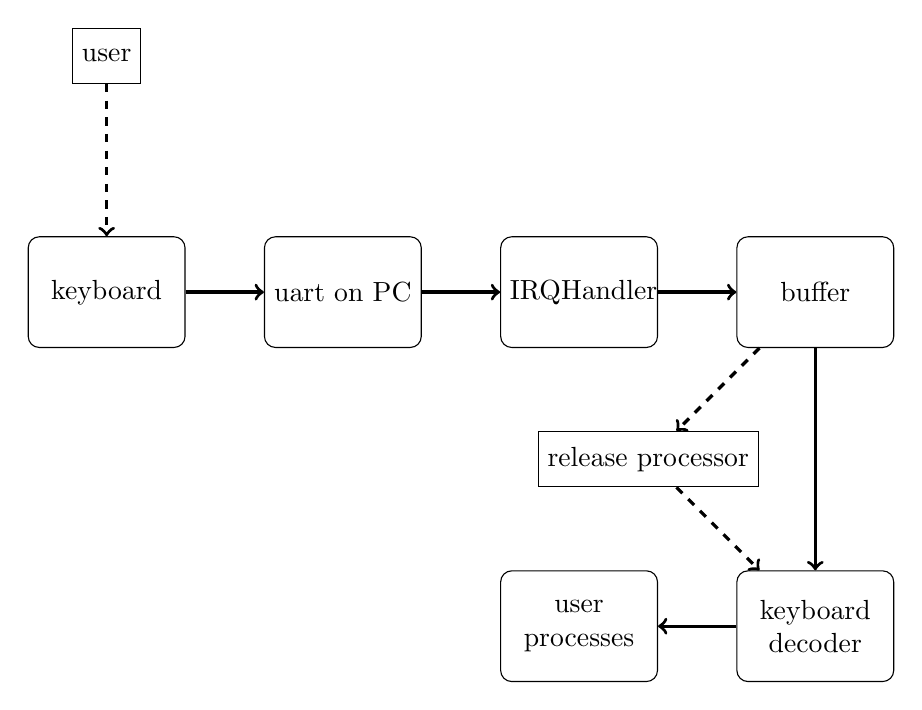
\begin{tikzpicture}[node distance = 3cm, auto]
        \label{diagram:input}
        % Place nodes
        \node [block] (kbd) {keyboard};
        \node [cloud, above of=kbd] (user) {user};
        \node [block, right of=kbd] (uart) {uart on PC};
        \node [block, right of=uart] (uart_h) {IRQHandler};
        \node [block, right of=uart_h] (buffer) {buffer};
        % TODO: fix this graph. It's broken.
        \node [cloud, below left of=buffer] (release) {release processor};
        \node [block, below right of=release] (kcd) {keyboard decoder};
        \node [block, left of=kcd] (user_proc) {user processes};
        % Draw edges
        \path [->,very thick,line,dashed] (user) -- (kbd);
        \path [->,very thick,line] (kbd) -- (uart);
        \path [->,very thick,line] (uart) -- (uart_h);
        \path [->,very thick,line] (uart_h) -- (buffer);
        \path [->,very thick,line,dashed] (buffer) -- (release);
        \path [->,very thick,line,dashed] (release) -- (kcd);
        \path [->,very thick,line] (buffer) -- (kcd);
        \path [->,very thick,line] (kcd) -- (user_proc);
    \end{tikzpicture}

{
% TODO: Format this. It's ugly.
\label{code:uart_input}
\begin{lstlisting}
------------------------------------------------------
crt.c:
------------------------------------------------------
__asm void UART0_IRQHandler() {
    ...
    BL c_UART0_IRQHandler
    ...
}
void c_UART0_IRQHandler {
    ...
    mark message as seen
    uart_receive_char_isr(newChar);
    ...
}
void uart_receive_char_isr(newChar) {
    if ((writeIndex + 1) % bufferSize == readIndex) {
        bufferOverflow = true
        return;
    }
    buffer[writeIndex] = newChar;
    writeIndex = (writeIndex + 1) % bufferSize
}
------------------------------------------------------
proc.c:
------------------------------------------------------
uint32_t releaseProcessor() {
    ...
    processUartInput();
    ...
}
void k_processUartInput() {
    ...
    lineBuffer = []
    while (buffer != null && readIndex != writeIndex) {
        char new_char = buffer[readIndex];

        readIndex = (readIndex + 1) % bufferSize;

        if (new_char == '\r') {
            kcdEnvelope = acquireMemoryBlock();

            kcdEnvelope = MT_KEYBOARD;

            kcdEnvelope->messageData = clone(buffer);

            k_sendMessage(kcdEnvelope, KEYBOARD_PID, KEYBOARD_PID);

            kcdEnvelope = NULL;
            continue;
        } else if (new_char == SHOW_DEBUG_PROCESSES) {
            Envelope *currentEnv = currentProcess->envelope;
            char *buf = NULL;

            buf = currentEnv->messageData;

            write(buf, "Allocated " + numSuccessfulAllocs + "b");

            currentEnv->messageType = MT_KEYBOARD;
            send currentEnv to CRT_PID

            for (procId : procIds) {
                Envelope *tempEnvelope = NULL;
                PCB *process = &(processes[i]);

                tempEnvelope = process->debugEnv;
                buf = tempEnvelope->messageData;

                writeProcessInfo(buf, process);

                sendMessage(tempEnvelope, CRT_PID, CRT_PID);
            }
            continue;
        }
    }
    ...
}
\end{lstlisting}
}
\section{Output}
    Output in our OS operates much more simply than output in a production-grade
    operating system.
    At a basic level, user processes send messages to the CRT process, which
    buffers the stream. The method ``uart\_send\_char\_isr'' consumes the buffer
    and sends it through UART to the putty on the PC. Additionally, the same
    ``UART0\_IRQHandler'' used in Input triggers ``uart\_send\_char\_isr'' when
    appropriate. Diagram \ref{diagram:output} is an over-simplification of the
    process that agrees with this description.

    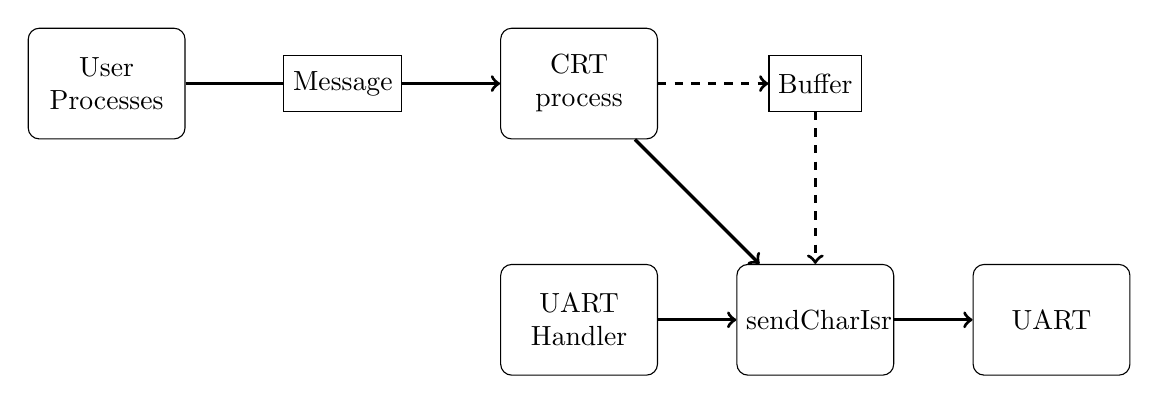
\begin{tikzpicture}[node distance = 3cm, auto]
        \label{diagram:output}
        % Place nodes
        \node [block] (user_proc) {User Processes};
        \node [cloud, right of=user_proc] (message) {Message};
        \node [block, right of=message] (crtProc) {CRT process};
        \node [cloud, right of=crtProc] (buffer) {Buffer};
        \node [block, below of=crtProc] (handler) {UART Handler};
        \node [block, right of=handler] (sendChar) {sendCharIsr};
        \node [block, right of=sendChar] (uart) {UART};
        % Draw edges
        \path [very thick,line] (user_proc) -- (message);
        \path [very thick,line] (user_proc) -- (message);
        \path [->,very thick,line] (message) -- (crtProc);
        \path [->,very thick,line] (crtProc) -- (sendChar);
        \path [->,very thick,line,dashed] (crtProc) -- (buffer);
        \path [->,very thick,line,dashed] (buffer) -- (sendChar);
        \path [->,very thick,line] (handler) -- (sendChar);
        \path [->,very thick,line] (sendChar) -- (uart);
    \end{tikzpicture}

    We decided to implement a larger feature set than required from the
    application specification in order to make our interface feel like a real
    command line. Our features include a text input bar that stays at the bottom
    while users type, coloured text, backspace support, and a few other
    enhancements.

    To achieve this, we save the buffered keyboard input into an envelope
    that belongs to a ``CRTData'' object. Whenever the buffer is cleared by a
    user pressing the ``enter button'', we move the cursor upwards, and write
    the content of the buffer in the cleared space. By shifting the cursor's
    position, we are able to maintain the currently buffered user text at the
    bottom of the screen, allowing the user to see their text as they enter it.
    Implementing deletion only required parsing a special character in a similar
    way to a hotkey.

\chapter{Misc}
% Make sure to include pseudocode and testing, if appropriate.

\section{Bridge Layer}

\part{User-level Processes}

\chapter{Proc 1}

\chapter{Proc 2}

\part{Lessons Learned}
% They call this the lessons learned summary.
% 1-2 pages
% what you did do well, both technically and organizationally, and what you
% would do differently if you were to do it again

\end{document}
